\setcounter{page}{1}

\section{\label{sec:The global biodiversity crisis} The global biodiversity
  crisis}

%Initial paragraph about ecosystems and biodiversity
Based on our current understanding, life on Earth appears to be unique in the
Universe. Its existence is the result of a long evolutionary process that
started around 3.5 billion years ago \cite{Taylor_1993,Schopf2006},
producing a wide variety of life forms. From the simplest unicellular organisms
to the most complex multicellular forms, the diversity of life is so vast that
it is estimated that there are around 9 million species of living beings in our
planet \cite{Cardinale2012}. This biodiversity is the result of the interaction
among organisms and with their environment, which has led to the development of
complex ecosystems. Ecosystems are the basic units of life on Earth, where
organisms interact with each other and with the environment, forming a
self-regulating system that is capable of maintaining life \cite{Levin2005}.
As Simon Levin eloquently describes \cite{Levin2005}:

\begin{displayquote}
  ``\textit{Ecosystems and the biosphere are complex adaptive systems, in which
    pattern
    emerges from, and feeds back to affect, the actions of adaptive individual
    agents, and in which cooperation and multicellularity can develop and
    provide
    the regulation of local environments, and indeed impose regularity at
    higher
    levels. The history of the biosphere is a history of coevolution between
    organisms and their environments, across multiple scales of space, time,
    and
    complexity.}''
\end{displayquote}

% Paragraph on the importance of biodiversity -- ecosystem services
Besides its intrinsic value, biodiversity is essential for the proper
functioning of ecosystems \cite{Gamfeldt2008}, which in turn provide
fundamental services to humankind. These services, known as ecosystem services,
include the production of oxygen, the regulation of climate, the provision
of food and water, and many others \cite{Daily1997}. Beyond these fundamental
life-supporting benefits, biodiversity also plays critical roles in nutrient
cycling and soil formation, processes integral to the sustainability of our
agricultural systems. The diversity of plant and animal life contributes to
robust ecosystems that can withstand and recover from a variety of disasters,
thereby ensuring ecological resilience. Moreover, biodiversity supports
recreational and tourism industries, which are significant sources of income
for many communities worldwide. The aesthetic and cultural values provided by
diverse ecosystems foster mental and physical health, and contribute to the
cultural heritage of communities, enriching our experience of the world.
Without services ecosystems provide, the stability of environments that support
human life would be greatly diminished, leading to profound economic and social
consequences.

% Paragraph on biodiversity loss, the biodiversity crisis
Unfortunately, the diversity of life on Earth is dramatically diminishing
\cite{Hughes1997,Ceballos2002,Pereira2010}, posing a serious threat to the
stability of ecosystems and the services they provide. Nowadays, wildlife
extinction rates are estimated to be 100 to 1000 times higher than the natural
background rate \cite{Ceballos2015,Pimm2014}, and up to 50\% of higher
taxonomic groups are already critically endangered \cite{Smith2009}. In the
last 50 years, the global population of vertebrates has declined by 69\%, about
50\% of the corals have disappeared due to different causes and roughly 10
million hectares of forests are lost annualy \cite{WWF2022}. Sadly, one could
continue listing more examples of biodiversity loss, but the point is clear: we
are facing a global biodiversity crisis. Indeed, this has led some scientists
to propose that we are entering the sixth mass extinction event in Earth's
history \cite{Barnosky2011}. However, unlike the natural extinction events in
Earth’s past, the current crisis is precipitated by only one species: humans.
As ecosystems falter and species vanish, the intricate web of life that
sustains economies, food security, and our very existence is at risk. If left
unchecked, the repercussions of this biodiversity crisis may lead to ecosystems
so impaired that they no longer fulfill their roles, fundamentally altering the
living conditions on our planet.

\begin{figure}[H]
  \centering
  \includegraphics[width=\textwidth]{Figures/biodiversity_intactness_index.pdf}
  \caption[The Biodiversity Intactness
    Index]{\label{fig:biodiversity_intactness_index} \textbf{The Biodiversity
      Intactness Index (BII).} The BII is a measure of the relative intactness
    of biodiversity in	different regions of the world. The index ranges from 0
    to 100, with higher values indicating higher levels of biodiversity
    intactness. In this map, the darkest red color represents BII$<50$,
    indicating that less than half of the original biodiversity remains in
    these regions. Data from \cite{Newbold2016}}
\end{figure}

% Paragraph on the drivers of biodiversity loss
The main drivers of global biodiversity loss, as identified in the Millennium
Ecosystem Assessment \cite{MEA2005}, encompass a range of
direct impacts on the natural world, most of which are caused by human
activities. Habitat change, exemplified by the rapid deforestation in the
Amazon Rainforest, results in drastic reductions in biodiversity by stripping
away the complex web of life supported by these environments
\cite{Laurance2012}. Climate change brings about shifts in temperature and
precipitation patterns that are markedly altering habitats. For instance, polar
regions are shrinking, threatening ice-dependent species with extinction
\cite{Post2013}, while ocean acidification is disrupting marine ecosystems by
impairing the ability of calcifying organisms to build their shells and
skeletons \cite{kroeker2013impacts}. Indeed, climate change may be a major
threat to global biodiversity in the next 100 years
\cite{Thomas2004,Loarie2009,Pimm2009,Warren2013,Warren2018}, with
predictions for species loss ranging from as low as 0\% to as high as 54\%
\cite{Urban2015}. Invasive species, such as the zebra mussel in North America,
can disrupt ecosystems by outcompeting native species, leading to changes in
the structure of the food webs, affecting the quality and quantity of primary
production, and causing diseases, which probably have been underestimated as an
ecological force \cite{Strayer2010}. Overexploitation of natural
resources, as seen in the overfishing of the world's oceans, can lead to the
collapse of entire ecosystems, as well as the loss of valuable food sources for
human populations \cite{Dayton1995,Coleman2002}. Finally, wildlife emergent
diseases threaten global biodiversity by potentially producing catastrophic
declines in new and not adapted host populations. If the diseases become
endemic, initial depopulation may be followed by chronic population depression,
which could even lead to local extinction \cite{Daszak2000}.

% Pollution, particularly from
% plastics, infiltrates marine ecosystems globally, endangering marine life
% through ingestion and entanglement, and highlighting the pervasive reach of
% human waste \cite{Rochman2015}.

In addition, all these drivers are interconnected and can have cascading
effects
on ecosystems \cite{Mora2007}. For example, climate change can expand the range
of invasive species, which in turn can produce emerging diseases that affect
native populations. Because native species have not co-evolved with the
pathogens producing these diseases, they are more susceptible to them, leading
to population declines and even extinctions \cite{Daszak2000}. Similarly,
ocean acidification is expected to reduce the calcification rates of corals,
making them more susceptible to diseases, bleaching events and
overexploitation, which can lead to the collapse of entire reef ecosystems
\cite{Hoegh-Guldberg2007}. These interactions among drivers of biodiversity
loss can produce synergistic effects that amplify the impacts on ecosystems,
making them more vulnerable to further disturbances and less resilient to
recover from them.

% Concluding paragraph
The global biodiversity crisis is a complex and multifaceted problem that
requires urgent action to prevent further loss of species and ecosystems. The
impacts of biodiversity loss are far-reaching, affecting not only the natural
world but also human societies and economies. To address this crisis, we need
to understand the underlying causes of biodiversity loss, predict the effects
of environmental changes on ecosystems, and develop effective strategies for
conservation. This requires a holistic approach that considers the interactions
among species and with the environment, as well as the dynamics of ecosystems
at different scales. In this context, complex systems science provides a
powerful framework to address these challenges.

\section{\label{sec:Complex systems in Ecology} Complex systems in Ecology}

% Paragraph complex systems in Ecology
Complex systems are composed of many interacting components
whose collective features cannot be understood by simply studying the
individual units in isolation \cite{Bianconi_2023}. The behavior of
complex systems arises from the interactions among the components, which can
lead to the formation of patterns, structures, and dynamics that are not
present at the individual level. This emergent behavior is a hallmark of
complex systems and illustrates how new properties and behaviors can arise from
relatively simple interactions when viewed at a larger scale. As a common
example, the flocking behavior of birds or schooling in fish is an emergent
property of the interactions among the individuals, where each follows simple
rules to maintain cohesion with its neighbors, leading to the formation of
complex patterns at the flock level \cite{Vicsek1995}.

Complex systems are also characterized by other features that are ubiquitous in
Ecology, such as non-linear dynamics, feedback loops, self-organization, a lack
of central control, pattern formation, unpredictability linked to the presence
of chaos and the presence of multiple temporal, spatial or organizational
scales \cite{Bianconi_2023}. Non-linear dynamics are extremely common in
ecological systems. An illustrative example are predator-prey interactions,
where changes in the population of prey can lead to non-proportional changes in
the population of predators, potentially causing oscillations rather than
steady states \cite{Lotka1925}. Self-organization is observed through the
spontaneous formation of spatiotemporal patterns that arise without any central
control, often mediated by scale-dependent feedback loops, like the formation
of vegetation patterns in arid ecosystems \cite{Rietkerk2008}. Contrary to
this spontaneous order, the presence of chaos in ecological systems can lead to
unpredictable dynamics related to the presence of chaos, as seen in the
population fluctuations of some species or the change of gene frequencies in
time \cite{May1974,May1976}. Overall, ecological processes operate across
multiple spatial, temporal and organizational scales, from local population
interactions to global biogeochemical cycles, in which each level influences
the others. Indeed, it is not surprising that the principles of complex systems
are that present in ecological systems, as they are composed of many
interacting units whose dynamics are shaped by the interactions among them and
with the environment. For example, ecosystems are composed of many species that
interact with each other and with the physical environment, forming intricate
food webs, nutrient cycles, and energy flows. And the same principles apply to
lower organizational levels such as populations, communities, and
metapopulations, where the interactions among individuals, species, and
habitats give rise to patterns and dynamics that are not always intuitive.

\begin{figure}[H]
  \centering
  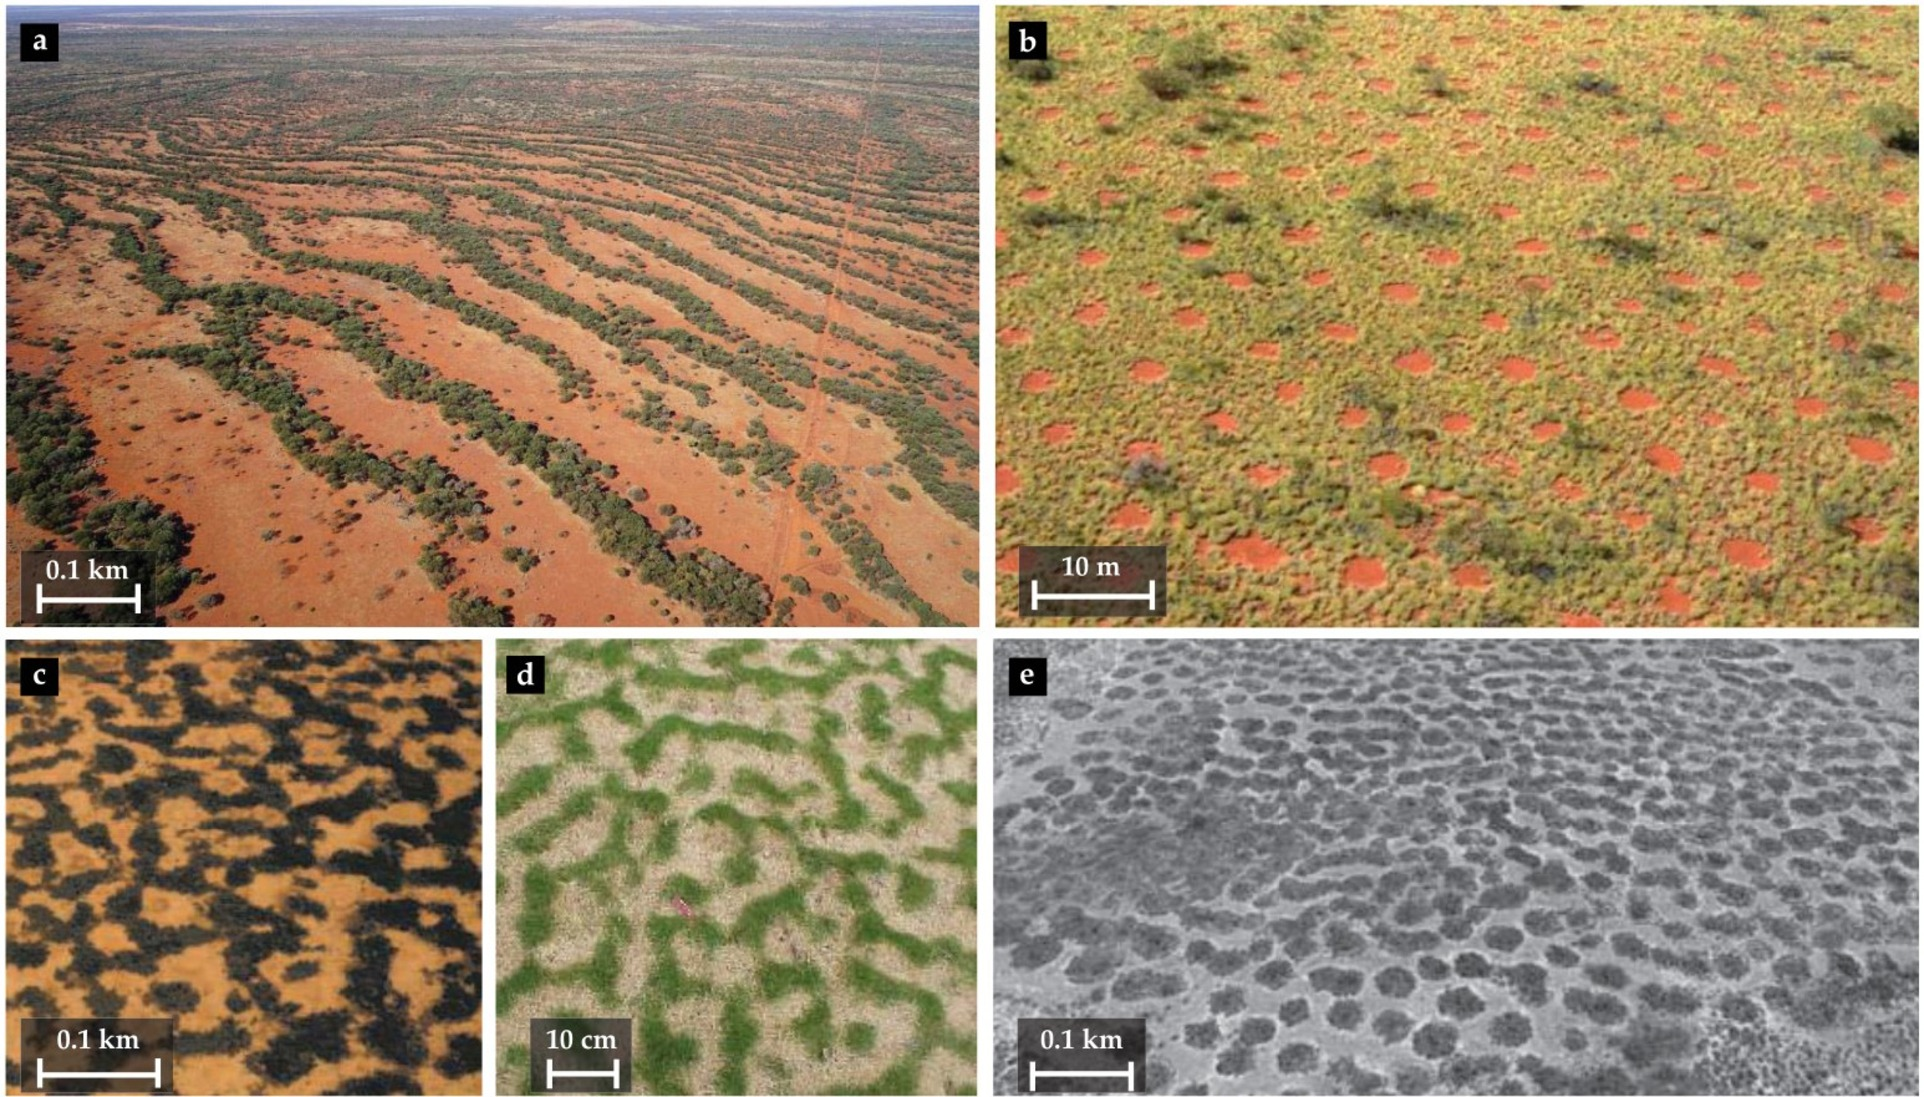
\includegraphics[width=\textwidth]{Figures/vegetation_patterns.jpg}
  \caption[Vegetation patterns in arid
    ecosystems]{\label{fig:vegetation_patterns} \textbf{Vegetation patterns in
      arid ecosystems.} These patterns are an example of self-organized
    structures that emerge from the interactions among plants and with the
    environment. These patterns optimize resource use and enhance ecosystem
    stability. Adapted from \cite{Ehud2019}}
\end{figure}

% Paragraph on the application of complex systems in Ecology
Complex systems approaches have become increasingly important in Ecology, not
only by providing theoretical frameworks to understand open questions in the
field, but also by posing new questions and challenges that were not previously
considered, thus expanding the discipline in new directions \cite{Milne1998}. A
major contribution of complex systems to Ecology is the theory of
self-organized systems, which provides a robust explanation for how
complex ecological patterns can emerge from simple local interactions without
the need for a centralized control mechanism. This principle has been
instrumental in deciphering the formation of highly ordered structures such as
the regular spacing in vegetation patterns, which optimize resource use in
challenging environments \cite{Tarnita2017}. Similarly, termite mounds are
examples of natural engineering, where collective behaviors lead to the
creation of sophisticated microhabitats that regulate temperature and humidity
essential for colony survival \cite{Heyde2021}. In marine environments, mussel
beds exhibit emergent properties such as enhanced stability and ecosystem
engineering through their aggregation behavior, significantly affecting
sediment dynamics \cite{Koppel2008}.

Scaling relationships are another key concept in complex systems that have
profound implications for understanding ecological patterns and processes.
Scaling laws describe how the properties of biological or ecological systems
change in a statistically regular way as function of a parameter, temporal or
spatial scale, organizational level or all of them. These laws, when approached
from a complex systems perspective, reveal underlying principles that govern
biological or ecological diversity across different scales, providing a
mathematical framework to unify patterns that span across the tree of life. A
well-known example is that of the allometric scaling laws in Biology, where
metabolic rates, growth patterns, and lifespan are shown to scale with the size
of organisms in a predictable way (e.g. Kleiber's Law, $BMR \propto M^{3/4}$,
where $BMR$ is the Basal Metabolic Rate and $M$ is the mass of the organism)
\cite{Peters1983}. For long time, these scaling laws were considered as
biological curiosities, until a mathematical framework was developed to explain
these patterns, showing that this impressive regularity arises from the
fractal-like structure of the organismns vascular system and the invariant size
of capilalries under the assumption of minimal energy expenditure
\cite{West1997}. Similar approaches can be followed to explain scaling
relationships in ecological systems, including population density, resource
distribution, and ecosystem productivity \cite{Brown2004}. Now these scaling
laws are recognized as fundamental principles that underlie the structure and
function of organisms. Indeed, there is an entire field of Ecology, known as
Macroecology, devoted to the study of these empirical patterns and the
mechanistic processes that generate them \cite{Brown1995Macroecology}.

% Paragraph on the role of models in Ecology
Is it clear that one of the key tools used in the study of complex systems in
Ecology is mathematical and computational modelling. Models are simplified
representations of reality that capture the essential features of a system,
allowing us to understand its dynamics, predict its behavior, and test
hypotheses about its functioning. Models can be used to explore the
consequences of different scenarios, design experiments, and inform management
decisions. In Ecology, models have been used to study a wide range of topics,
from population dynamics and community interactions to ecosystem processes and
global biogeochemical cycles.

\section{\label{sec:Mathematical and computational models} Mathematical and
  computational models}

Mathematical and computational models have become pivotal in modern ecology,
offering profound insights into the dynamics of complex ecological systems.
These models serve as essential tools for simulating and understanding how
ecosystems function, interact, and respond to various environmental pressures
\cite{HOCH19983}. At their core, these models translate biological and
ecological processes into mathematical descriptions, which can be manipulated
and studied under controlled, repeatable conditions. This approach allows
ecologists to test hypotheses about ecological interactions and processes in a
virtual environment, where real-world experimentation would be either
impractical or impossible. In addition, models provide a means to explore the
consequences of different management strategies, predict the outcomes of
environmental changes, and assess the impacts of human activities on
ecosystems. Overall, mathematical and computational models are indispensable
tools for advancing ecological research and have have been recognised as some
of the most powerful approaches to guide empirical work and provide a framework
for synthesis, analysis, development of conservation plans and policy making
\cite{levin1992mathematics,Murray_book,sarkar2006biodiversity}

One of the simplest and most widely used types of models in ecology are
deterministic continuous-time models, such as ordinary differential equations
(ODEs), which describe how the state of a system changes over time based on
known biological or ecological processes. ODEs usually represent \textit{mean
  field} descriptions of the system under study, assuming that the population
or community is well-mixed and that the interactions among individuals are
homogeneous. Under these assumptions, the system can be described by
\textit{rate equations} that capture the dynamics of the system in terms of
rates of change of the state variables. These models have been used to study a
wide range of ecological processes, from population growth and competition to
predator-prey dynamics and disease transmission, providing valuable insights
into the mechanisms that drive the dynamics of ecological systems
\cite{Murray_book}.

Obviously, continuous-time models are not the only way to model the dynamics of
ecological systems. Discrete-time models, such as difference equations, are
also widely used in Ecology. Perhaps the logistic map, which describes the
growth of a population over discrete generations, is by far the most famous
example \cite{May1974}. Indeed, this model led to the discovery of
\textit{chaotic dynamics} in simple ecological systems, in which small changes
in the initial conditions can lead to large differences in the long-term
behavior of the system. This discovery revolutionized the field of Ecology,
highlighting the importance of non-linear dynamics in population and community
dynamics. Of course, this chaotic behavior is not exclusive to discrete-time
models, as it can also be observed in continuous-time models, such as the
Lotka-Volterra predator-prey equations, which exhibit complex dynamics, such as
limit cycles, bifurcations, and chaos, under certain parameter values
\cite{Murray_book}.

However, deterministic models may not fully capture the inherent variability
and uncertainty present in ecological systems, which is not always due to
chaotic dynamics. Stochastic models can provide a more realistic representation
of the randomness and variability that are present in some ecological systems.
For example, stochastic differential equations (SDEs) extend ODEs by including
random fluctuations in the system that represent the effects of environmental
variability, demographic stochasticity, or genetic drift. Similarly, discrete
stochastic models simulate the dynamics of ecological systems by modeling the
interactions among individuals as discrete events that occur with a certain
probability. These models have been used to study the effects of environmental
noise on population dynamics, the persistence of species in fluctuating
environments, and the spread of diseases \cite{Murray_book}.

The dynamics of ecological systems are not only determined by their internal
processes, but also by the spatial structure of the environment in which they
are embedded. The natural extension of continuous-time models to
incorporate spatial dynamics is the use of partial differential equations
(PDEs), which describe how the state of a system changes over time and
space \cite{Murray_book}. These models have been instrumental in exploring
dispersal mechanisms and predict changes in population density across space.
PDEs are also used to model the spread of invasive species and disease
transmission through susceptible populations, providing insights into the
impacts of spatial structure on ecological invasions \cite{tilman1997spatial}.
In addition, nonlinear PDEs lead to pattern formation, the spontaneous
emergence of spatial structure in systems with suitable local interaction and
spatial coupling terms, like in the case of the Turing mechanism
\cite{turing1952chemical}.

Environmental or demographic noise can also be incorporated into these models
by means of stochastic partial differential equations (SPDEs), which provide a
more realistic representation of the variability and uncertainty present in
spatially structured ecological systems. Of course, spatial models can also
be discrete, such as cellular automata, which divide the environment into
discrete cells that can change state over time based on a set of rules. These
models have been used to study the spread of forest fires, the dynamics of
vegetation patterns, and the formation of spatially structured populations,
providing insights into the effects of local interactions on the dynamics of
ecological systems. Overall, spatial models are particularly valuable in
conservation planning, helping to determine the most effective configurations
of habitats to preserve species diversity and ecological function.

Both these continuous and discrete models can be used to study the dynamics of
ecological systems, but they are often limited by their assumptions of
homogeneity in interactions and spatial structure. Network models and
individual-based models (IBMs) provide frameworks for studying more complex and
heterogeneous interactions, both in a spatially extended and non-spatial
context. Network models describe the interactions between the entities under
study as a network of nodes and edges, where nodes represent individuals or
populations and edges represent the interactions between them. These models
have been used to study the structure and dynamics of various ecological
networks, such as food webs and pollination networks, and provide a rich
framework to tackle problems in which interactions among many species are
central, such as coevolution in species-rich communities \cite{Bascompte2007}.
Of course, network models can be both deterministic or stochastic.

IBMs simulate the behaviors of individual organisms or entities based on a set
of simple rules. These models are exceptionally useful to study heterogeneous
populations, in which individuals differ in their characteristics or behaviors,
and spatially explicit interactions. IBMs help in understanding how individual
heterogeneity contribute to group dynamics and ecosystem-level patterns,
providing insights that are often obscured in more traditional approaches.
Initially, IBMs were used to model forest succession, exemplified by the JABOWA
model, which described tree community dynamics in response to shading and
growth patterns. Their applications then expanded to animal populations,
including fish recruitment, bird nesting colonies, and predator-prey
interactions, allowing for the examination of complex interspecific
relationships and behaviors \cite{deangelis2014}.

% Machine learning and ecological modeling
Data-driven techniques such as Machine Learning (ML) are also increasingly
being used in ecological modeling. These methods, are particularly useful for
handling complex, high-dimensional data and capturing non-linear relationships.
In short, ML algorithms learn how to predict an output variable from input data
by iteraively adjusting their parameters to minimize the error between the
predicted and observed values. Machine learning models have been widely used to
predict species distributions and habitat suitability from environmental
variables, providing valuable insights into the impacts of climate change on
biodiversity \cite{Christin2019}. More recently, deep learning models, a
subfield of ML based on artificial neural networks, have shown promise in
ecological applications, such as identifying species in camera trap images
\cite{Tabak2019} or classifying the behaviour of animals captured in images and
videos \cite{Christin2019}. Specifically, the conjuntion of deep learning
models with remote sensing data is revolutionizing the field of landscape
ecology, allowing to monitor land cover changes \cite{Kussul2017}, map canopy
height \cite{Lang2023}, track animal migrations \cite{Wu2023} or detect plant
diseases \cite{Zarco-Tejada2021}. As computational capabilities continue to
grow, and as datasets become more comprehensive and accessible, the potential
for mathematical and computational models in ecology expands. This progression
promises not only to deepen our understanding of ecological systems but also
improve our ability to predict and mitigate the impacts of human activities and
environmental changes on the natural world.

This is only a brief overview of the wide range of mathematical and
computational models that have been developed and applied in Ecology. The
diversity of models reflects the complexity of ecological systems and the
diverse questions that ecologists seek to answer. By combining theoretical
insights with empirical data, mathematical and computational models provide a
powerful framework for understanding the dynamics of ecological systems,
predicting their responses to environmental changes, and informing management
decisions. In the following chapters, we will explore how these models can be
used to address some of the most pressing challenges in Ecology and
Conservation Biology, from the spread of infectious diseases to the decline of
important ecosystems under global change.

\section{\label{sec:Thesis structure} Thesis structure}

This thesis is devoted to develop theoretical and data-driven methods to
address timely problems in Ecology and Conservation Biology from the
perspective of Complex Systems. We tackle a variety of current challenges
related to biodiversity loss caused by climate change and emergent diseases,
including expanding vector-borne plant diseases, Mass Mortality Events (MMEs)
produced by marine diseases, ocean acidification, and the decline of important
coastal ecosystems like coral reefs or seagrass meadows. To address these
challenges, we developed a series of theoretical and data-driven models that
integrate ecological theory, data analysis, mathematical models, computational
simulations, and artificial intelligence. The thesis is structured as follows.
In Chapter 2, we present the theoretical framework and scientific background
that underpins the research presented in this thesis. We review basic concepts
of infectious disease modelling and disease biogeography, explain the main
methods used in the data-driven approaches and present the context of the
ecological systems that will be studied in the following chapters. The main
results of the thesis are divided into four parts, each formed by several
chapters. In \cref{part:nacras}, we focus on the development of theoretical
models to understand the dynamics of marine diseases and their impacts on
marine ecosystems, exemplified by the Mass Mortality Event of \textit{Pinna
  nobilis}. Similarly, in \cref{part:VBD}, we develop theoretical models to
study the vector-borne plant diseases in which the vector population is
non-stationary and non-periodic. Our framework is then applied to diseases
caused by the bacterium \textit{Xylella fastidiosa}. In \cref{part:PD_risk}, we
develop and apply a climate-driven epidemic model to predict the risk of
establishment of \textit{Xylella fastidiosa} diseases globally, both in current
and future climates. In \cref{part:data-driven}, we develop data-driven models
to address complex ecological problems, such as the decline of coral reefs and
seagrass meadows or ocean acidification. Finally, in \cref{part:discussion}, we
summarise our contributions, present the main conclusions of the thesis and
discuss the implications of our results for the conservation of biodiversity
and the management of ecosystems under global change.